\chapter{Convolutional Neural Network Architecture for Feature Extraction}
\label{sec:cnnarchitecture}

We implement a Convolutional Neural Network architecture that takes $28 \times 28 \times 1$ grayscale pixel images as input and predicts the probability of a data sample for each of the ten classes (five classes for learning subsets and two classes for learning even and odd numbers). We use the following architecture for our MNIST and Omniglot experiments, where we adapt the output size of the \textit{dense\_2} layer depending on the amount of classes for the MNIST data. For Omniglot, we have to invert the images first and scale from $105 \times 105$ pixels to $28 \times 28$ pixels.

\begin{figure}[H]
    \centering
    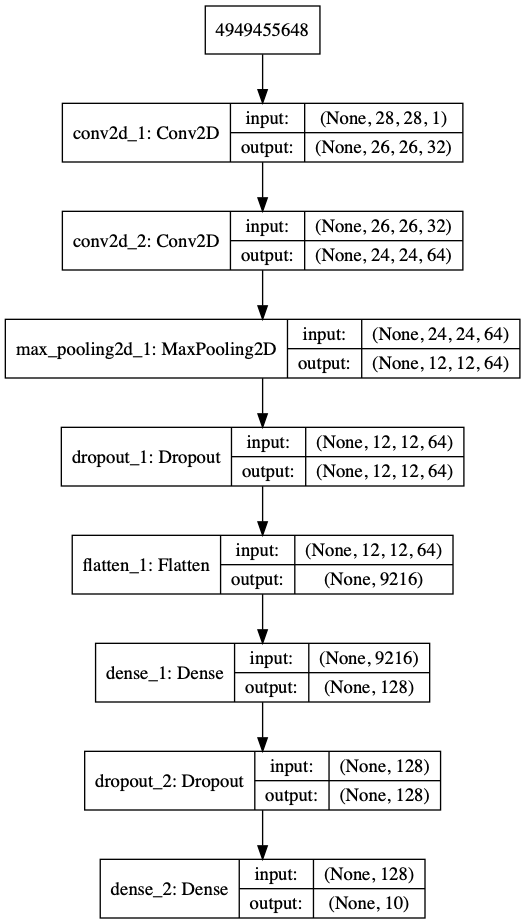
\includegraphics[width=0.45\textwidth]{images/model}
    \caption{We use a small Convolutional Neural Network (CNN) architecture to create meaningful features for the MNIST and the Omniglot data.}
    \label{fig:model}
\end{figure}